\part{AI architectures}
\frame{\partpage}

\begin{frame}{Rule-based AI}
	Generally implemented as \texttt{if} statements or event-based triggers
\end{frame}

\begin{frame}{Finite state machines}
	\begin{center}
		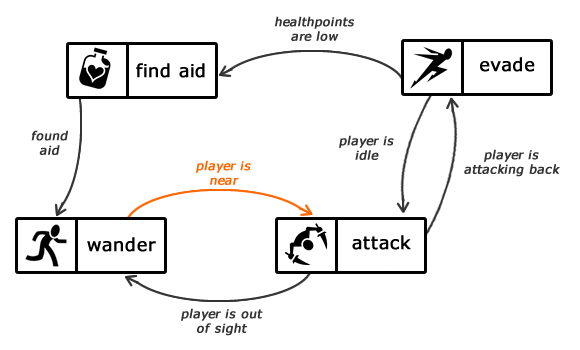
\includegraphics[width=\textwidth]{fsm_enemy_brain}
		% https://gamedevelopment.tutsplus.com/tutorials/finite-state-machines-theory-and-implementation--gamedev-11867
	\end{center}
\end{frame}

\begin{frame}{Behaviour trees}
	\begin{center}
		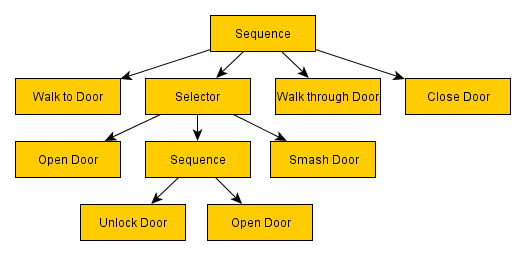
\includegraphics[width=\textwidth]{behaviour_tree}
		% https://www.gamasutra.com/blogs/ChrisSimpson/20140717/221339/Behavior_trees_for_AI_How_they_work.php
	\end{center}
\end{frame}

\begin{frame}{Game tree search}
	\begin{center}
		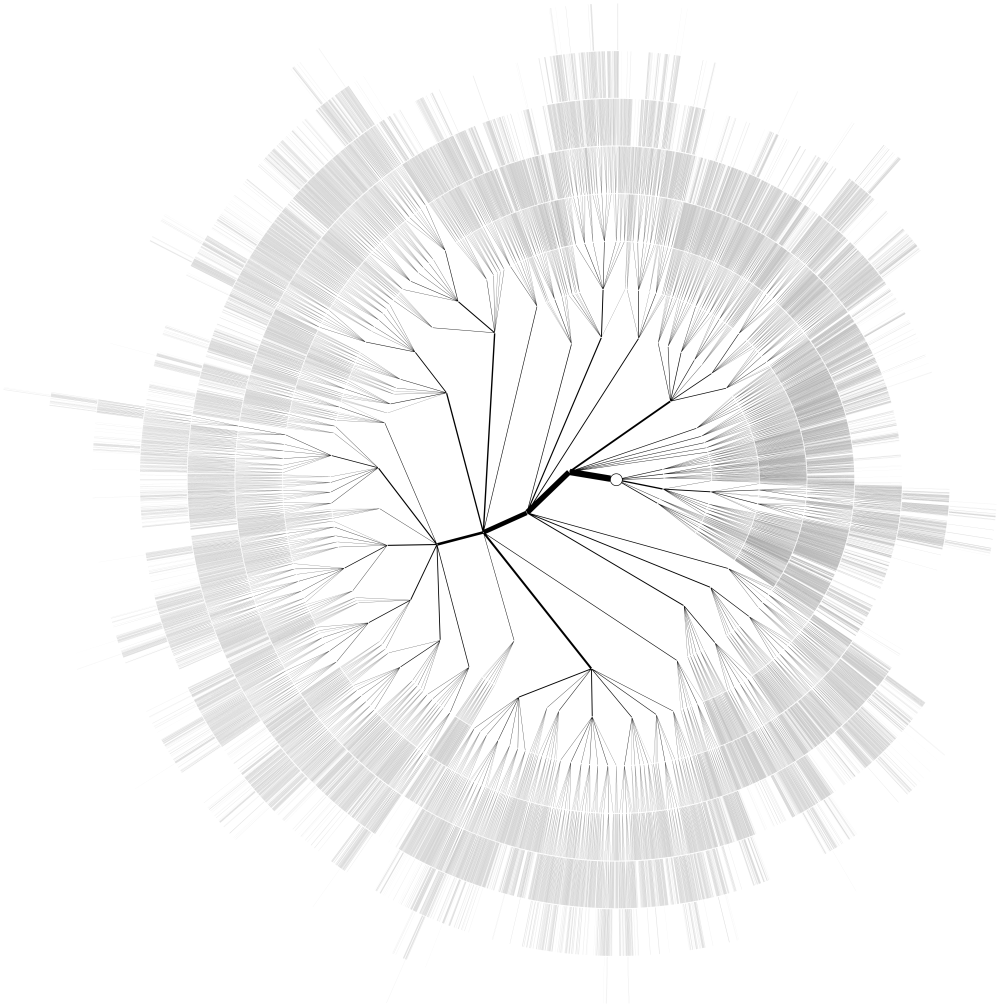
\includegraphics[height=0.7\textheight]{mcts}
	\end{center}
\end{frame}

\begin{frame}{Multi-agent approaches (e.g.\ flocking)}
	\begin{center}
		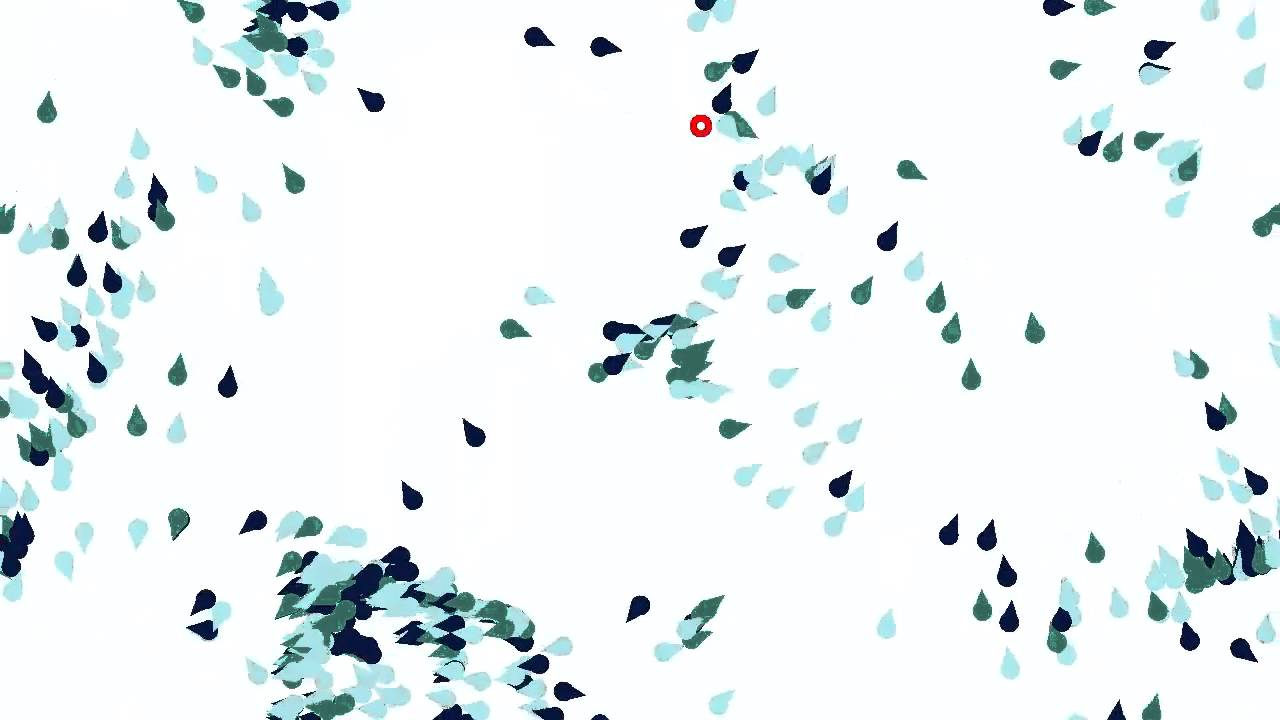
\includegraphics[width=\textwidth]{flocking}
		% https://www.youtube.com/watch?v=5p6OAEVKw-0
	\end{center}
\end{frame}

\begin{frame}{Machine learning}
	\begin{center}
		\colorbox{white}{
			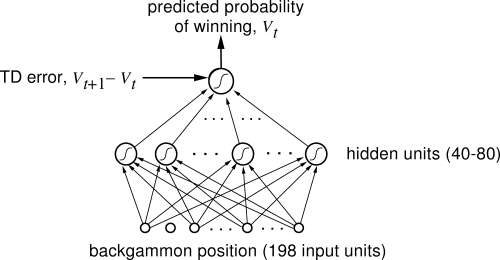
\includegraphics[width=0.7\textwidth]{tdgammon}
		}
		% https://users.auth.gr/kehagiat/Research/GameTheory/12CombBiblio/BackGammon.html
	\end{center}
\end{frame}

\begin{frame}{AI architectures}
	\begin{itemize}
		\pause\item Can roughly be divided into \textbf{hand-authored}...
			\begin{itemize}
				\pause\item Rule-based, FSM, behaviour trees
			\end{itemize}
		\pause\item ... and \textbf{computational intelligence}
			\begin{itemize}
				\pause\item Search, multi-agent, machine learning
			\end{itemize}
		\pause\item Do you want to \textbf{design} the AI behaviours yourself,
			or do you want them to \textbf{emerge} from the system?
		\pause\item Predictability and authorial control versus adaptability and novelty
		\pause\item Can also combine the two
			\begin{itemize}
				\pause\item E.g.\ use a rule-based system to constrain a CI system
				\pause\item E.g.\ flocking --- individual agents are usually rule-based, but overall flock dynamics
					are emergent
			\end{itemize}
	\end{itemize}
\end{frame}
